\chapter{Experiments}



%\begin{wrapfigure}{l}{8cm}
%\vspace{-0.5cm}
%\begin{centering}
%\subfigure[Training mistakes vs b]{\includegraphics[width=0.27\textwidth]{figs/mnist1-eps-converted-to.pdf}\label{fig:mnist1}}
%\subfigure[Test error vs no. of queries]{\includegraphics[width=0.27\textwidth]{figs/mnist2b-eps-converted-to.png}\label{fig:mnist2}}
%\caption{Left: mean of fraction no. of mistakes SHAMPO made during training time on MNIST of all examples and only queried. Right: test error vs no. of queries is plotted for all MNIST one-vs-one problems.}
%\end{centering}
%%\vspace{-0.3cm}
%\end{wrapfigure}


We evaluated the SHAMPO algorithm using four different datasets: USPS, MNIST (both OCR), Vocal Joystick 
(VJ, vowel recognition) and document classification (NLP). 
The USPS dataset, contains $7,291$ training examples and $2,007$ test examples, each one of them is a 
$16\times16$ pixels gray-scale images converted to a $256$ dimensional vector. 
The MNIST dataset with $28\times28$ gray-scale images, contains $60,000$ 
examples in the training set and $10,000$ in the testing set. In both cases there are $10$ possible labels,
the $0$ to $9$ digits. The VJ project was built to enable individuals with motor impairments to use vocal
 parameters to control objects on a computer screen (buttons, sliders, etc.) and ultimately 
 electro-mechanical instruments (e.g., robotic arms, wireless home automation devices). The VJ tasks is to 
 predict a vowel from eight possible vowels. Each example is a frame of spoken value described with $13$ 
 MFCC coefficients transformed into 26 features. There are $572,911$ training examples and $236,680$ test 
 examples. We created binary tasks from these multi-class datasets using two reductions: One-vs-Rest 
 setting and One-vs-One setting. For example, in both USPS and MNIST there are $10$ binary one-vs-rest 
 tasks and $45$ binary one-vs-one tasks.  The NLP document classification is one-vs-one  binary 
 classification include of spam filtering, news items and news-group classification, sentiment classification, 
 and product domain categorization. A total of $36$ binary prediction tasks over all, with a total of 
 $252,609$ examples, and input dimension varying between $8,768$ and $1,447,866$. 
 Details of the individual binary tasks can be found elsewhere~\cite{Crammer:2012:CLC:2343676.2343704}.
This yielded seven collections (USPS, MNIST and VJ; each as one-vs-rest or one-vs-one) and document 
classification.

\section{Hard and Easy Tasks }
First, we wanted to show that indeed, the SHMAPO algorithms are optimal for different distributions of hard and
 easy tasks and also tasks from different domains and dimensions. For that reason, we created an eighth 
 collection, named MIXED, which consists of $40$ tasks: $10$ random tasks from each one of the four 
 basic datasets (one-vs-one versions). Now, from each one of the eight dataset collections we generated 
 between $6$ to $10$ combinations (or problems), each problem was created by sampling between 
 $2$ and $8$ tasks which yielded a total of $64$ multi-task problems. 
We tried to diversify problems difficulty by including both hard and easy binary classification problems.
For example, from the VJ dataset we generated 10 multitask problems with up to 5 tasks each, and different 
number of hard and easy tasks : 1 (easy task) + 1 (hard task), 1+2, 1+3, 1+4, 2+1, 2+2, 2+3, 3+1, 3+2, 4+1.
The hardness of a binary problem is evaluated by the number of mistakes the Perceptron algorithm performs 
on the problem where for each multitask problem, we sample uniformly from each group of tasks 
(hard and easy) .

We evaluated two baselines as well as our algorithm. Algorithm {\em uniform} picks a random task to be 
queried and updated (corresponding to $b\rightarrow\infty$), {\em exploit} which picks the tasks with the 
lowest absolute margin (i.e. the ``hardest instance''), this combination corresponds to $b \approx 0$ of 
SHAMPO. We tried for SHAMPO $13$ values for $b$, equally spaced on a logarithmic scale between 
$10^{-7}$ and $10^{5}$. 
All algorithms made a single pass over the training data.  We ran two versions of the our First Order algorithm: 
plain version, without aggressiveness (updates on mistakes only, $\lambda=0$) and an 
Aggressive version $\lambda=b/2$ (we tried lower values of $\lambda$ as in the bound, 
but we found that $\lambda=b/2$ gives better results), both with uniform prior ($a_i=1$). 
We used separate training set and a test set, to build a model and evaluate it.

The results are evaluated using $2$ quantities. First, the average test error (over all the dataset combinations) 
and the average score. For each combination we assigned a score of $1$ to the algorithm with the lowest 
test error, and a score of $2$, to the second best, and all the way up to a score of $6$ to the algorithm with 
the highest test error.



\begin{table}[h] 
\begin{centering}
\caption{Test errors percentage . Scores are shown in parenthesis.}
\label{tab:table1}
{\scriptsize	
\begin{tabular}{|l|r|r|r|r|r|r|}
\hline
                         & \multicolumn{3}{c|}{\textbf{Aggressive $\lambda=b/2$}}               & \multicolumn{3}{c|}{\textbf{Plain}}                 \\ \hline
\textit{Dataset}         & \textit{exploit} & \textit{SHAMPO}         & \textit{uniform} & \textit{exploit} & \textit{SHAMPO} & \textit{uniform} \\ \hline
{VJ 1 vs 1 }        & 5.22 (2.9)       & \textbf{4.57 (1.1)}   & 5.67 (3.9)       & 5.21 (2.7)       & 6.93 (4.6)    & 6.26 (5.8)       \\
\textrm{VJ 1 vs Rest}    & 13.26 (3.5)      & \textbf{11.73 (1.2)} & 12.43 (2.5)      & 13.11 (3.0)        & 14.17 (5.0)     & 14.71 (5.8)     \\
\textrm{USPS 1 vs 1}      & 3.31 (2.5)       & \textbf{2.73 (1.0)}     & 19.29 (6.0)        & 3.37 (2.5)       & 4.83 (4.0)      & 5.33 (5,0)         \\
\textrm{USPS 1 vs Rest}  & 5.45 (2.8)      & \textbf{4.93 (1.2)}  & 10.12 (6.0)        & 5.31 (2.0)         & 6.51 (4.0)      & 7.06 (5.0)         \\
\textrm{MNIST 1 vs 1}     & 1.08 (2.3)       & \textbf{0.75 (1.0)}     & 5.9 (6.0)         & 1.2 (2.7)       & 1.69 (4.1)      & 1.94 (4.9)     \\
\textrm{MNIST 1 vs Rest} & 4.74 (2.8)      & \textbf{3.88 (1.0)}     & 10.01 (6.0)       & 4.44 (2.8)      & 5.4 (3.8)    & 6.1 (5.0)          \\
\textrm{NLP documents} & 19.43 (2.3)     & \textbf{16.5 (1.0)}     & 23.21 (5.0)        & 19.46 (2.7)     & 21.54 (4.7)  & 21.74 (5.3)     \\
\textrm{MIXED}           & 2.75 (2.4)       & \textbf{2.06 (1.0)}     & 13.59 (6.0)        & 2.78 (2.6)       & 4.2 (4.3)     & 4.45 (4.7)       \\ \hline
\textit{Mean score}      & (2.7)           & \textbf{(1.1)}       & (5.2)           & (2.6)           & (4.3)        & (5.2)           \\ \hline
\end{tabular}
}
\end{centering}
\vspace{-0.5cm}
\end{table}

Results  are summarized in \tabref{tab:table1}.  In general {\em exploit} is better than {\em uniform}
 (for majority of the datasets) and aggressive algorithm is better than non-aggressive one. 
 Aggressive SHAMPO yields the best results both evaluated as average 
(over tasks per combination and over combinations). Remarkably, even in the mixed dataset 
(where tasks are of different nature: images, audio and documents), the aggressive SHAPO improves over 
uniform (4.45\% error) and the aggressive-exploit baseline (2.75\%), and achieves a mean test error of 2.06\%.

Indeed, \tabref{tab:table1} shows that aggressive SHAMPO outperforms better alternatives. Yet, we claim that a 
good prior may improve results. We compute prior over the 45 USPS one-vs-one tasks and 10 
USPS one-vs-rest, by running the perceptron algorithm on $1000$ examples and computing the number of mistakes.  
We set the prior to be proportional to this number. We then reran aggressive SHAMPO with prior, 
comparing it to aggressive SHAMPO with no prior (i.e. $a_i=1$). 
The results are summarized in \tabref{tab:table2}. The prior improves performance in the USPS 1 vs 1 
collection and USPS 1 vs Rest, when evaluated using score-rank, on averaged it is slightly worse than 
aggressive SHAMPO with not prior.
Aggressive SHAMO with prior achieves average error of $1.47$ (vs. $2.73$ with no prior) on 1-vs-1 USPS 
and $4.97$ (vs $4.93$) on one-vs-rest USPS, with score rank of 1.0 (vs 2.9) and 1.7 (vs 2.0) respectively.
\figref{fig:tst_err_u1}  and \figref{fig:tst_err_ur} shows the test error for all values of $b$ we evaluated.
A good prior is shown to outperform the case $a_i=1$ for most values of $b$. 
Again, we chose a specific prior generator system, however, another method or 
another prior knowledge may lead to better results.

 \begin{table}[h]
   \begin{centering}
 \caption{Test errors percentage . Scores are shown in parenthesis.}
 \label{tab:table2}
 {\scriptsize	
 \begin{tabular}{|l|r|r|r|r|r|r|}
 \hline
                         & \multicolumn{3}{c|}{\textbf{Aggressive $\lambda=b/2$}}           & \multicolumn{3}{c|}{\textbf{Aggressive $\lambda=b/2$ with prior}}  \\ \hline
 \textit{Dataset}        & \textit{exploit} & \textit{SHAMPO}     & \textit{uniform} & \textit{exploit} & \textit{SHAMPO}        & \textit{uniform} \\ \hline
 {USPS 1 vs 1}     & 3.31 (3.9)       & 2.73 (2.9)        & 19.29 (5.6)      & 1.92 (2.2)       & \textbf{1.47 (1.0)}    & 17.66 (5.4)      \\
 {USPS 1 vs Rest} & 5.45 (3.5)       & \textbf{4.93 }(2.0) & 10.12 (5.7)     & 5.23 (2.8)      & 4.97 \textbf{(1.7)} & 9.64 (5.3)      \\ \hline
 \end{tabular}
 }
 \end{centering}
 \end{table}
 
 \figref{fig:bars1} and \figref{fig:bars2} show the test error of the three algorithms on two of document 
classification combinations, with four and eight tasks. Clearly, not only SHAMPO performs better, 
but it does so on each task individually. (Our analysis above bounds the total number of mistakes over all 
tasks.)
 
  \begin{figure}[h]
\begin{centering}
\subfigure[4 text classification tasks]{\includegraphics[width=0.45\textwidth]{figs/problem-9_4_2_2-1.eps}\label{fig:bars1}}
\subfigure[8 text classification tasks]{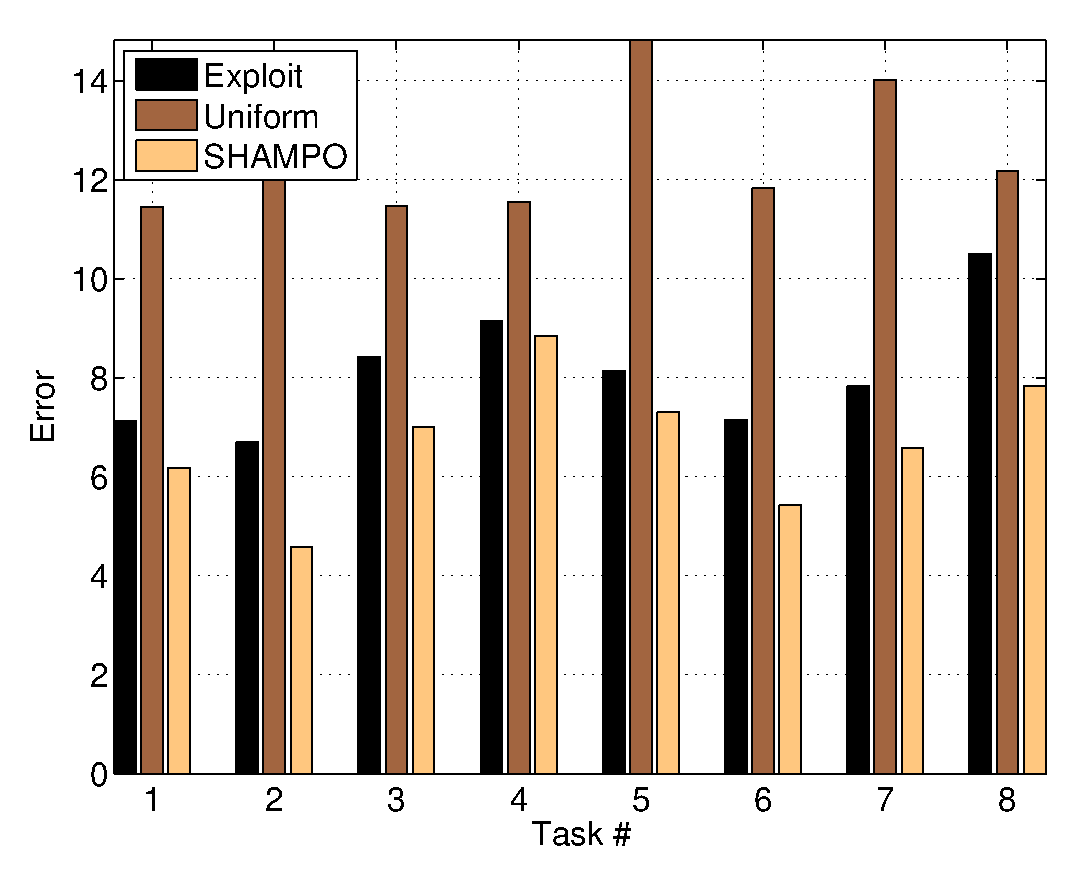
\includegraphics[width=0.45\textwidth]{figs/problem-9_4_4_4-1.eps}\label{fig:bars2}}
 \caption{
 Test error of aggressive SHAMPO on (a) four and (b) eight binary text classification tasks. 
 Three algorithms are evaluated: uniform, exploit, and aggressive SHAMPO with $\lambda=b/2$. }
\end{centering}
\end{figure}


\vspace{-0.1cm}
\section{Multi-task Binary Classification}
First, we evaluated all the mentioned variations of SHAMPO algorithms. We ran a 
single pass over all of the training examples for all datasets and $11$ equally spaced values of b 
between $10^{-5}$ and $10^5$. The algorithms performance was evaluated using 
mean of accumulated training error of all tasks and the mean of test errors over 
all of the tasks for each datasets. Since the NLP dataset doesn't have a test 
set, we evaluated those quantities using 4 cross validation folds. We repeated 
the experiments 100 times and took the mean of all algorithm runs.
For simplicity, we denote each one of those algorithms the  
abbreviations: First Order (FO), First Order AGgressive (AG) with two different values of $\lambda$, 
$\lambda = b/2$ and $\lambda = b/4$ , First Order with PRior (PR), First Order 
ADaptive (AD), Second Order (SO) and Second Order AGgressive (SOAG). 
Recall, in the adaptive algorithm the constant $b$ parameter is replaced with the constant 
$\beta$.

\figref{fig:train_errors} shows the mean cumulative training errors over all tasks. The behavior is similar for 
all of the datasets. We can see that as expected, in the exploration interval ($b\rightarrow\inf$) 
all the algorithms shows high error rate, where in the vast majority, this is 
also the highest error. In the exploitation interval ($b\rightarrow 0$), we  see 
lower cumulative error than the exploration case for the most of the datasets. 
This makes sense, since we query (and update) more on the harder tasks.
Between those two extreme cases, there is a point where cumulative error is 
lower. This point is where $b$ gets its optimal value. This value can change 
between datasets and algorithms and next we see a convenient experimental way to find it. 
There are algorithms and datasets (e.g. VJ one-vs-one in \figref{fig:tst_err_v1}), that this point converges
into the exploitation area, it may depends on the examples noise and the number of examples 
in the dataset. As we claimed before, a pure exploitation approach may not be the best choice, at least on 
the first online steps, especially for problem with small number of examples.
can see the same phenomena in \figref{fig:test_errors} which shows the mean 
test error for all tasks and all round for different $b$ values and different 
tasks. Here, we added one more algorithm, the Watch All algorithm (WA), which runs $K$ parallel online - 
perceptron algorithms, one per task, while each one of them query and watches all of the tasks labels, without any limitation on the feedback.
We show this algorithm here as a benchmark, to measure how much SHAMPO algorithms looses or gain 
performance with respect to the algorithm that can watch all the labels. 

Wen we compare all of the algorithms, there is no such absolute winner, however, 
it is obvious from results that the aggressive algorithms shows better 
performance than the rest of them. For most of the algorithms, the aggressive version of the second order (SOAG) seems to preform better 
then the rest. It is probably due to the fact that it draws tasks to query on, based on two measurements 
($r_{i,t} $ and $\hat{p}_{i,t}$) and also make an aggressive update. The second best algorithm is  
the first order aggressive algorithm (AG) which performs the best on a 
limited $b$ interval because the aggressiveness depends strongly on $b$. The 
first order algorithm with prior (PR) doesn't show an improvement over the ordinary first order (FO) algorithm. 
In fact, we already mentioned before than better prior may lead to an improvements in the results. 
The adaptive $b$ algorithm (AD), does not show an improvement over FO as well. 

Now, we focus on the tasks that the algorithm chooses to annotate on each iteration for various values 
of $b$. \figref{fig:queried} shows the total number of mistakes that first order SHAMPO  algorithm 
made during training time on all datasets. 
We show here two quantities: fraction of mistakes over all training examples (denoted by ``All tasks'' - blue) 
and fraction of mistakes over only queried examples (denoted by ``Queried tasks'' - dashed red). 
In pure exploration (large values of $b$) both quantities are the same, as the choice of task to be labeled 
is independent of the task and example, and essentially the fraction of mistakes in queried examples is a 
good estimate of the fraction of mistakes over all examples. 
The other extreme is when performing pure exploitation (low values of
$b$), here, the fraction of mistakes made on queried examples went up, while the overall fraction of mistakes 
went down. This indicates that the algorithm indeed focuses its queries on the harder inputs, which in turn, 
improves overall training mistake. There is a sweet point of $b$ (that is changed between datasets), for 
which SHAMPO is still focusing on the harder examples, yet reduces the total fraction of training mistakes even more. 
The existence of such tradeoff is predicted by \thmref{thm:FO_bound}.  
So far we saw algorithms and bounds that depends on the value 
of $b$ and proof that an optimal value 
that get a minimal accumulative train error exists. The inevitable question is: how to find such 
optimal value? We suggested an adaptive algorithm, yet, this algorithm have an 
initial value to set. Is there a practical way to find this value? Recall, the only prediction mistakes that the algorithm knows 
about, are the mistakes of the queried tasks. When we look at the accumulative mistakes that the algorithm 
made in  \figref{fig:queried}, it is possible to find an answer for this question.
The value of $b$ which minimizes the mean test error, is about the point for which there is a change in the error of 
queried examples (the only quantity SHAMPO observes), which provides a rough rule-of-thumb to pick 
$b$ automatically on-the-fly.

\begin{figure}[!ht]
\begin{centering}
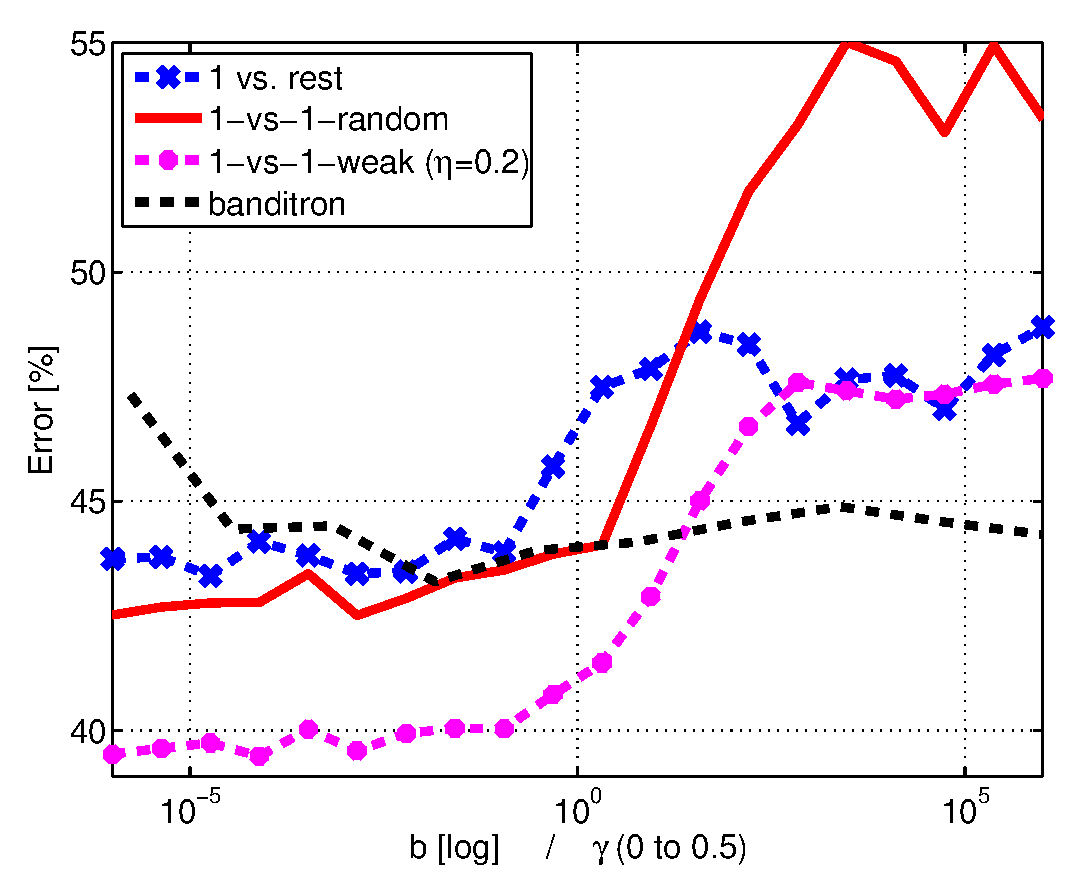
\includegraphics[width=0.7\textwidth]{figs/VJ_three_methods.eps}\label{fig:mc_vj}
\caption{Multi-class error on VJ data for three bandit reductions and the banditron.}
\end{centering}
\end{figure}

\begin{figure}[!htb]
\begin{centering}
\subfigure[MNIST one-vs-one]{\includegraphics[width=0.4\textwidth]{figs/queried-m1.eps}\label{fig:bars1}}
\subfigure[MNIST one-vs-rest]{\includegraphics[width=0.4\textwidth]{figs/queried-mr.eps}\label{fig:bars2}}
\subfigure[USPS one-vs-one]{\includegraphics[width=0.4\textwidth]{figs/queried-u1.eps}\label{fig:bars1}}
\subfigure[USPS one-vs-rest]{\includegraphics[width=0.4\textwidth]{figs/queried-ur.eps}\label{fig:bars2}}
\subfigure[VJ one-vs-one]{\includegraphics[width=0.4\textwidth]{figs/queried-v1.eps}\label{fig:bars1}}
\subfigure[VJ one-vs-rest]{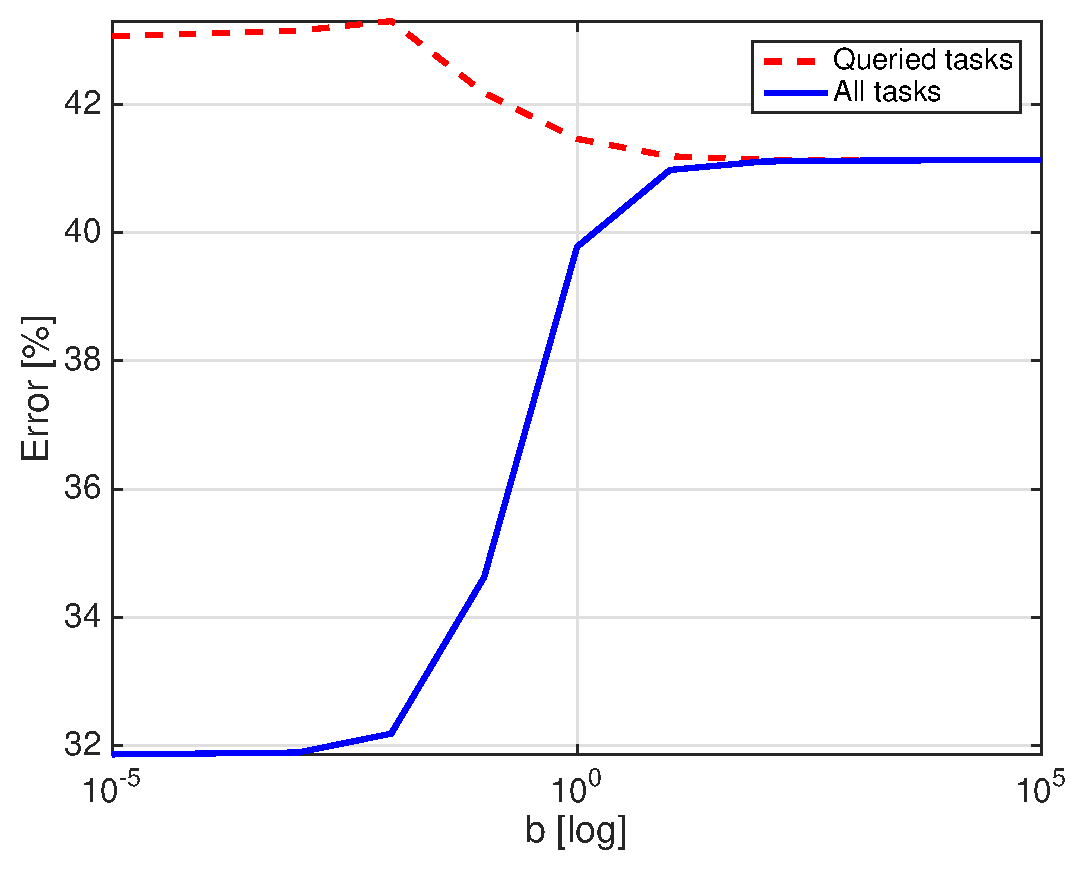
\includegraphics[width=0.4\textwidth]{figs/queried-vr.eps}\label{fig:bars2}}
\subfigure[NLP one-vs-one]{\includegraphics[width=0.4\textwidth]{figs/queried-n.eps}\label{fig:bars2}}
\caption{train error queried vs all -FO algorithm}
\label{fig:queried}
\end{centering}
\vspace{-0.5cm}
\end{figure}


Another perspective of the phenomena is that for values of $b\ll \infty$ SHAMPO focuses on the harder 
examples, is illustrated in \figref{fig:test_scatter} where test error vs number of queries is plotted for each 
task in all the datasets. We show three cases: uniform, exploit and a mid-value of $b\approx 0.01$ which 
tradeoffs exploration and exploitation. We take the MNIST one-vs-one data set as an example and 
refer a few points. First performing uniform querying, all 
tasks have about the same number of queries ($266$), close to the number of examples per problem 
($12,000$), divided by the number of problems ($45$). Second, when having a tradeoff between exploration 
and exploitation, harder problems (as indicated by test error) get more queries than easier problems. 
For example, the four problems with test error greater than $6\%$ get at least $400$ queries, which is 
about twice the number of queries received by each of the $12$ problems with test error less than $1\%$. 
Third, as a consequence, SHAMPO performs equalization, giving the harder problems more labeled data, 
and as a consequence, reduces the error of these problems, however, is not increasing the error of the 
easier problems which gets less queries (in fact it reduces the test error of almost all 45 problems!). 
The tradeoff mechanism of SHAMPO, reduces the test error of each problem by more than $40\%$ 
compared to full exploration. Fourth, exploits performs similar equalization, yet in some hard tasks it 
performs worse than SHAMPO. This could be because it overfits the training data, by focusing on 
hard-examples too much, as SHAMPO has a randomness mechanism.


 % In fact in the USPS dataset we found a good prior that can improves the performances.  In order to create this prior, we ran over the examples first simple perceptron algorithm with full feedback, and computes the prior as a fraction of the error from the initial run. The results are shown in \tabref{tab:table2} and as.  In addision, the results for the MIXED dataset support the claim that the tasks can comes from different fields and different dimensions.

\begin{figure}[!t]
\begin{centering}
\subfigure[MNIST one-vs-one]{\includegraphics[width=0.4\textwidth]{figs/test-m1.eps}\label{fig:tst_err_m1}}
\subfigure[MNIST one-vs-rest]{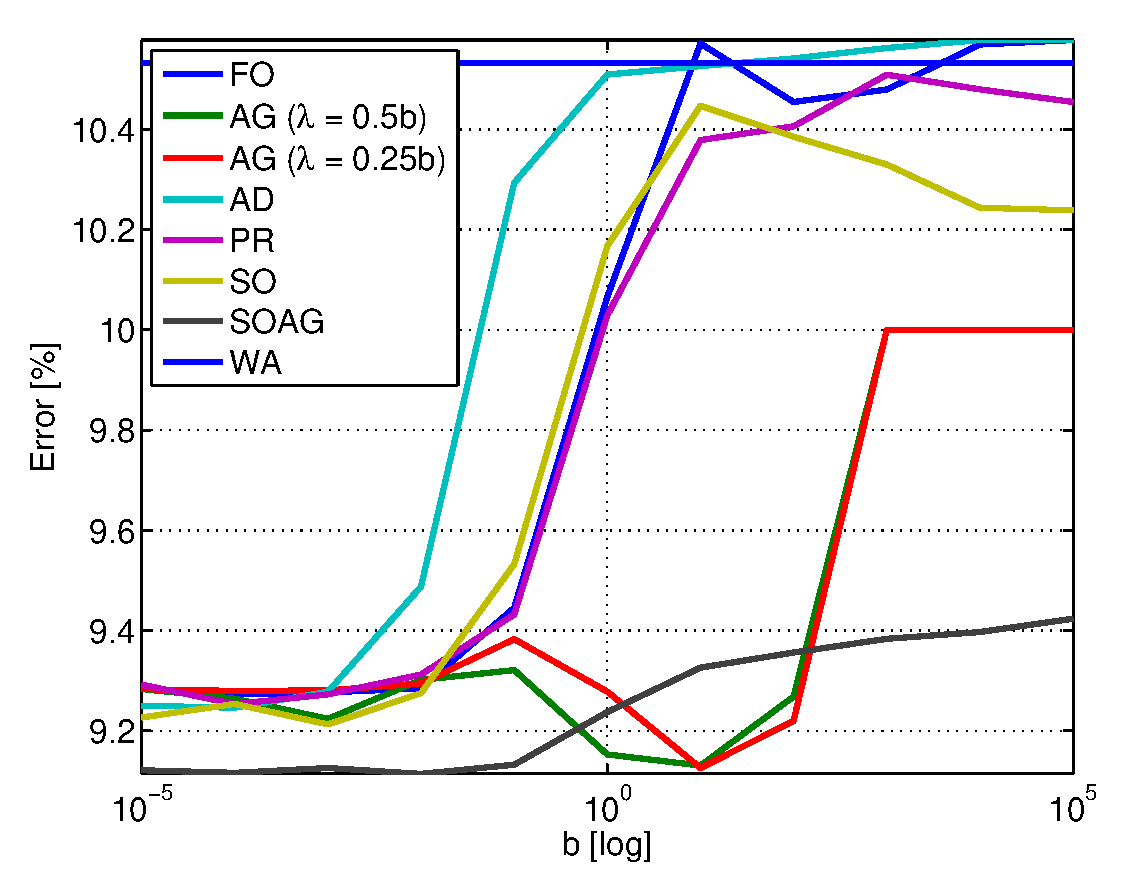
\includegraphics[width=0.4\textwidth]{figs/test-mr.eps}\label{fig:tst_err_mr}}
\subfigure[USPS one-vs-one]{\includegraphics[width=0.4\textwidth]{figs/test-u1.eps}\label{fig:tst_err_u1}}
\subfigure[USPS one-vs-rest]{\includegraphics[width=0.4\textwidth]{figs/test-ur.eps}\label{fig:tst_err_ur}}
\subfigure[VJ one-vs-one]{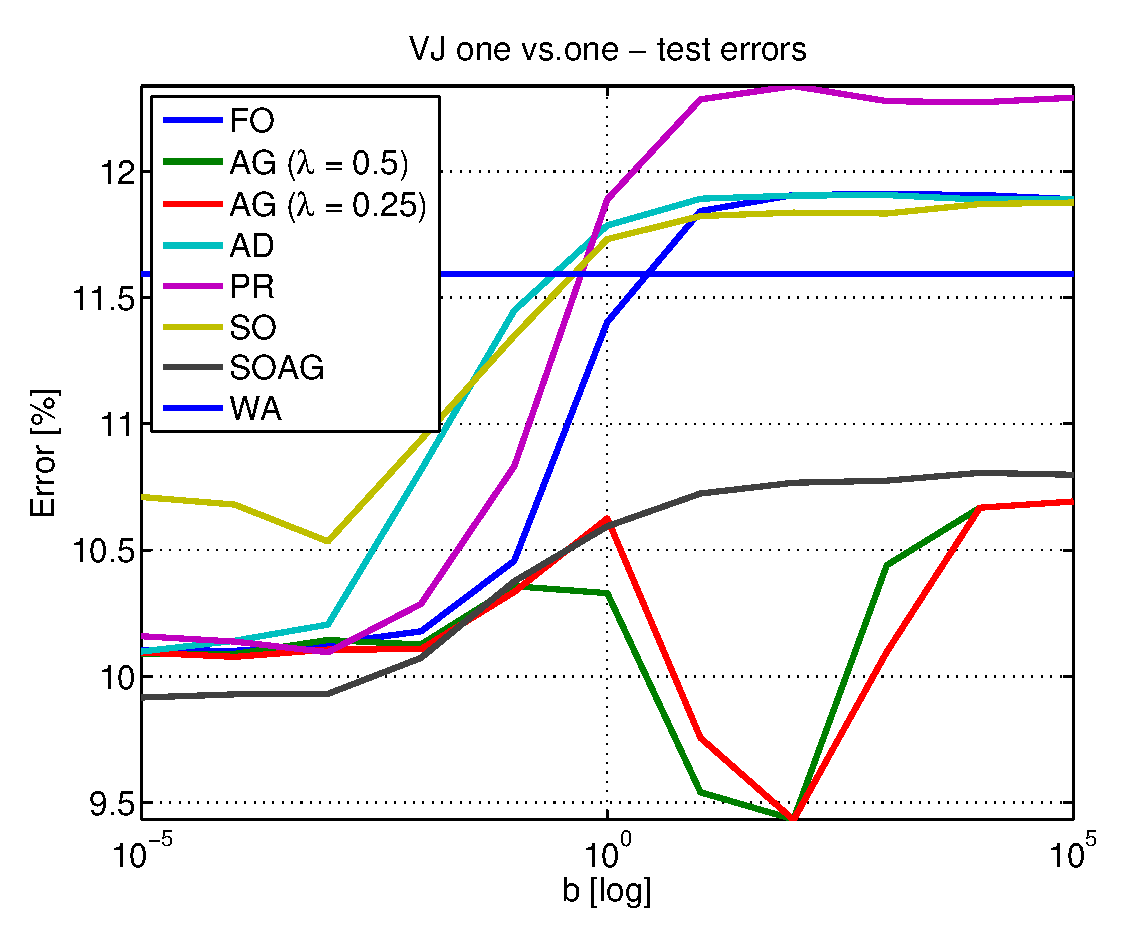
\includegraphics[width=0.4\textwidth]{figs/test-v1.eps}\label{fig:tst_err_v1}}
\subfigure[VJ one-vs-rest]{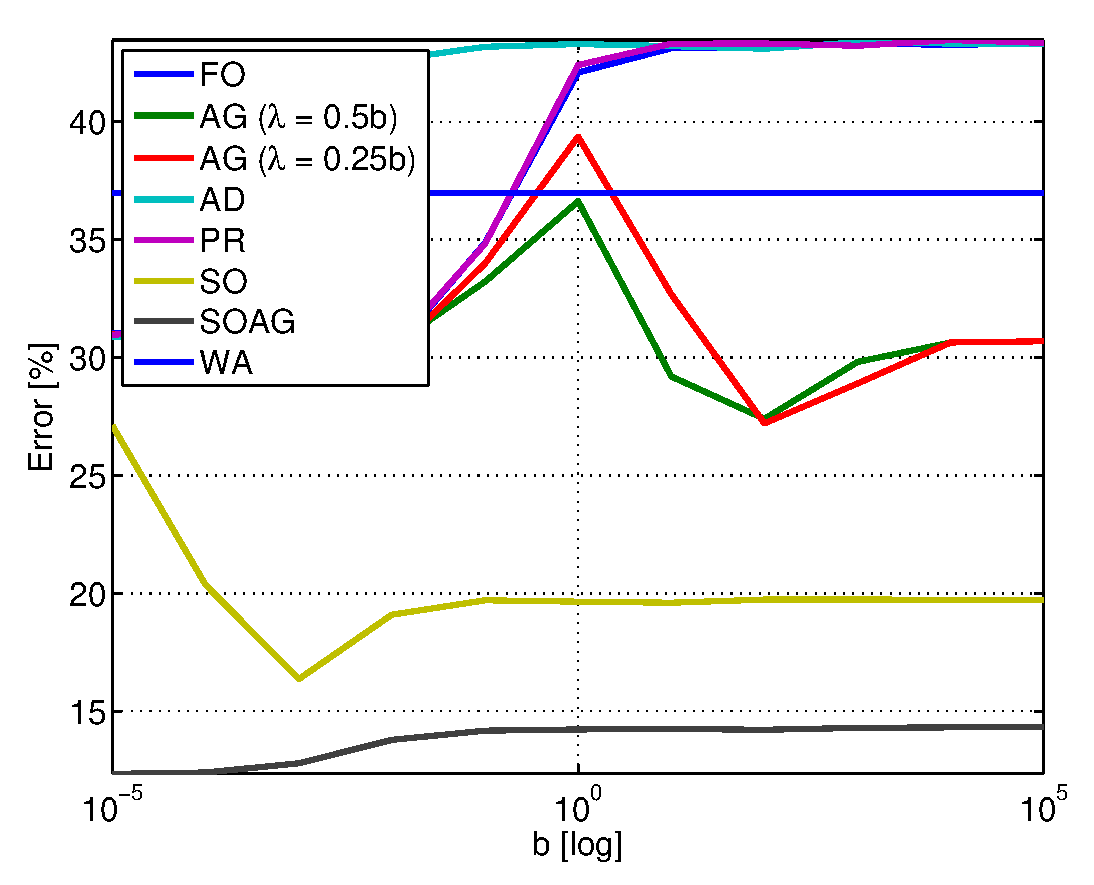
\includegraphics[width=0.4\textwidth]{figs/test-vr.eps}\label{fig:tst_err_vr}}
\subfigure[NLP ove-vs-one]{\includegraphics[width=0.4\textwidth]{figs/test-n.eps}\label{fig:tst_err_n}}
\caption{test error}
\label{fig:test_errors}
\end{centering}
\vspace{-0.5cm}
\end{figure}

\begin{figure}[!t]
\begin{centering}
\subfigure[MNIST one-vs-one]{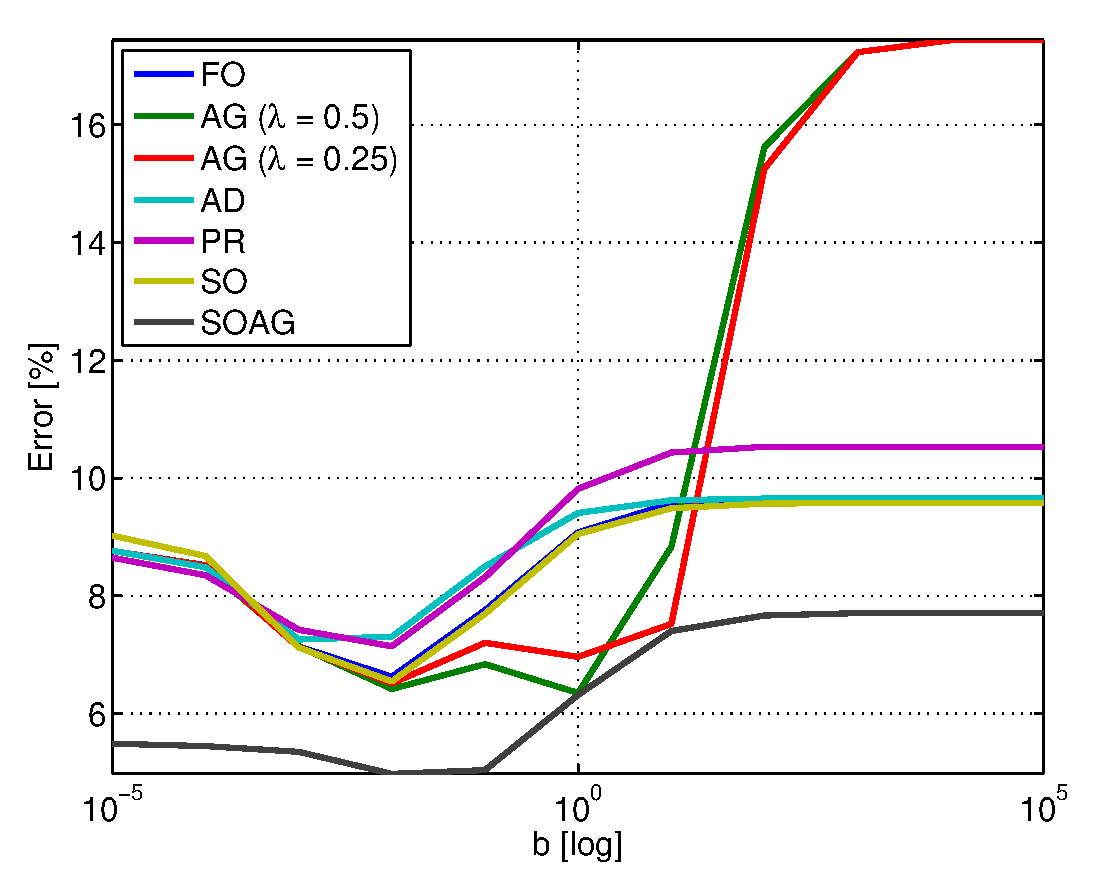
\includegraphics[width=0.4\textwidth]{figs/train-m1.eps}\label{fig:bars1}}
\subfigure[MNIST one-vs-rest]{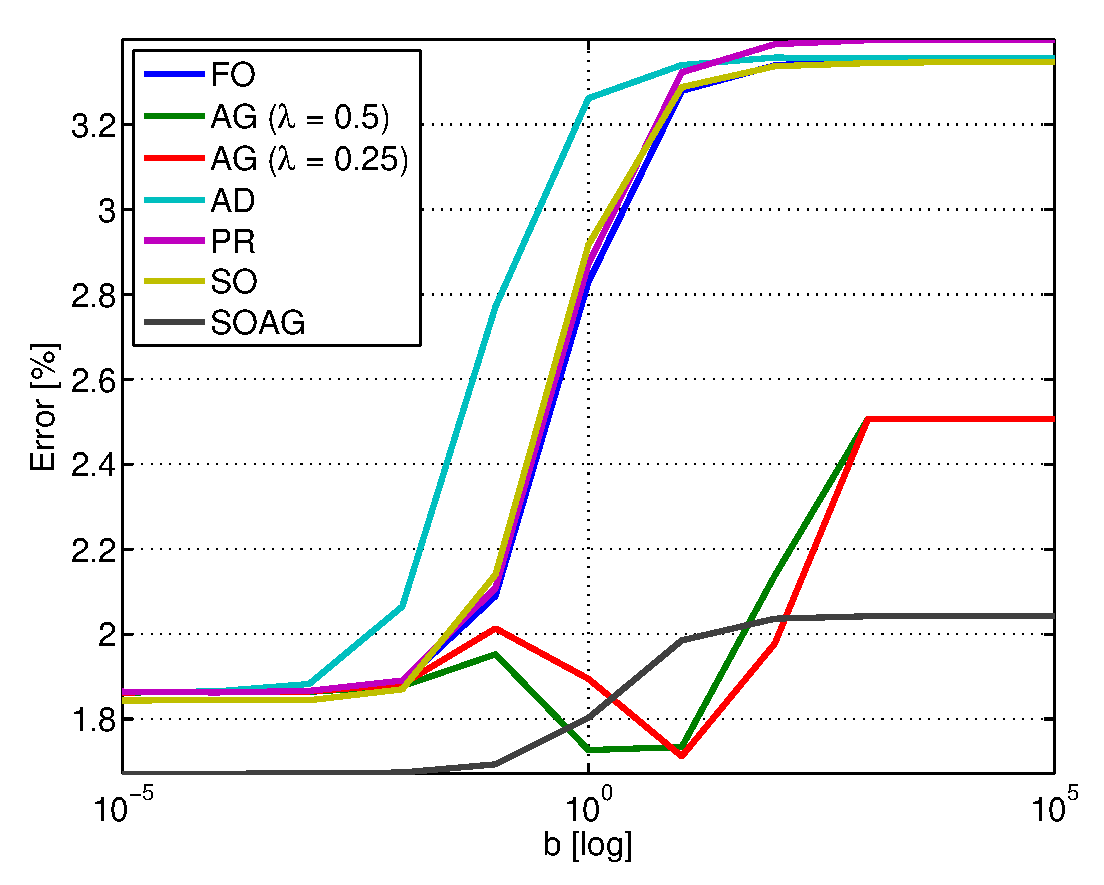
\includegraphics[width=0.4\textwidth]{figs/train-mr.eps}\label{fig:bars2}}
\subfigure[USPS one-vs-one]{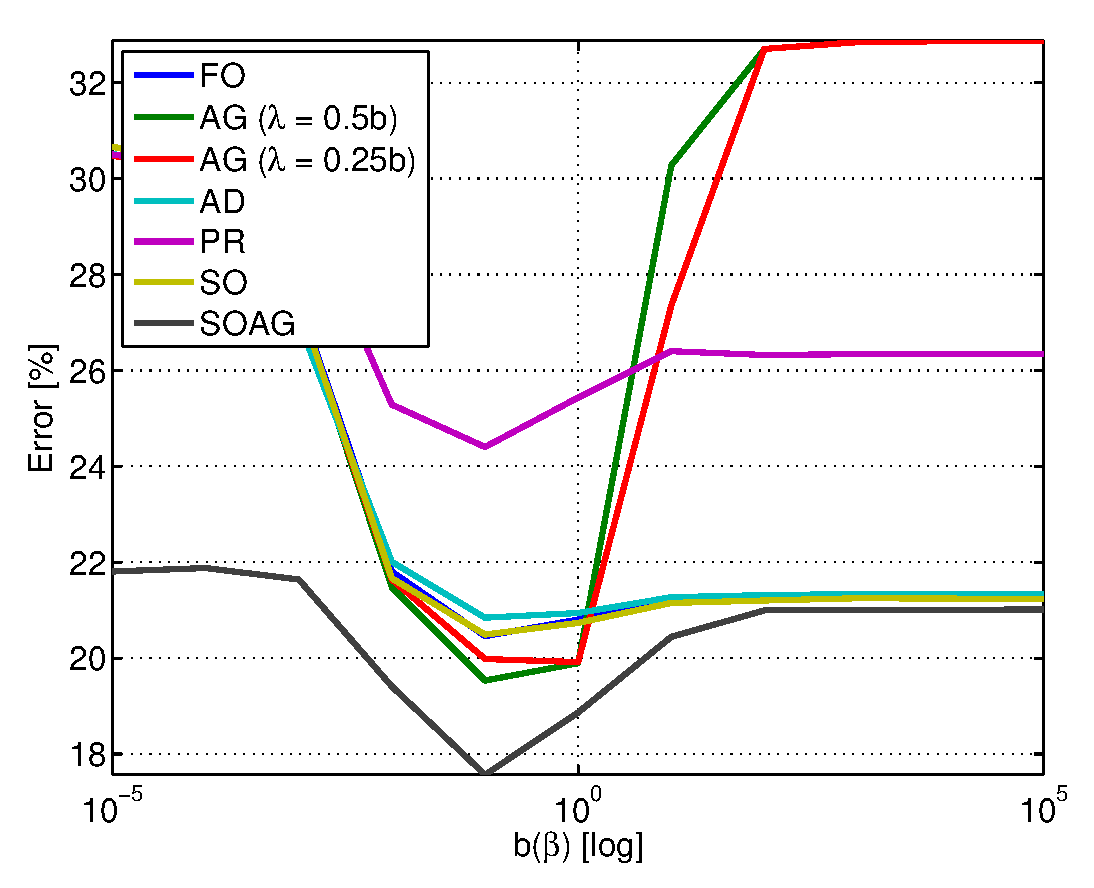
\includegraphics[width=0.4\textwidth]{figs/train-u1.eps}\label{fig:bars1}}
\subfigure[USPS one-vs-rest]{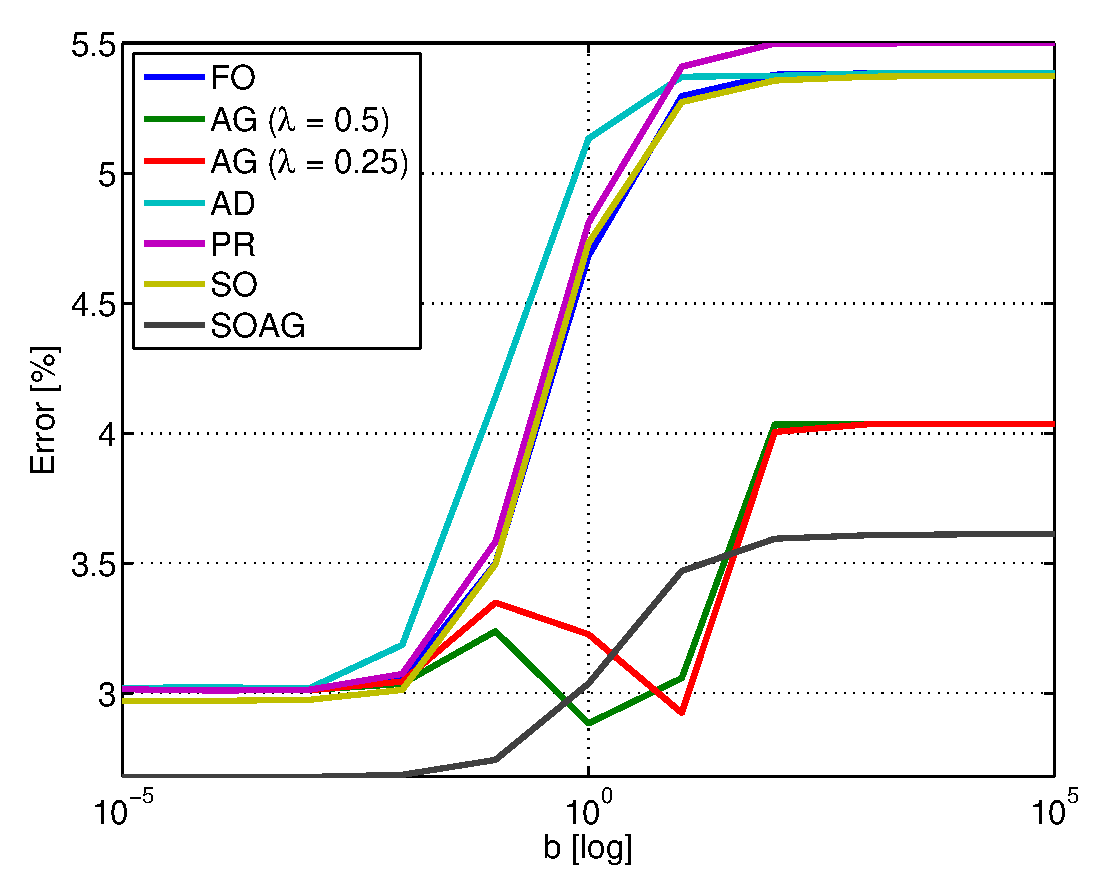
\includegraphics[width=0.4\textwidth]{figs/train-ur.eps}\label{fig:bars2}}
\subfigure[VJ one-vs-one]{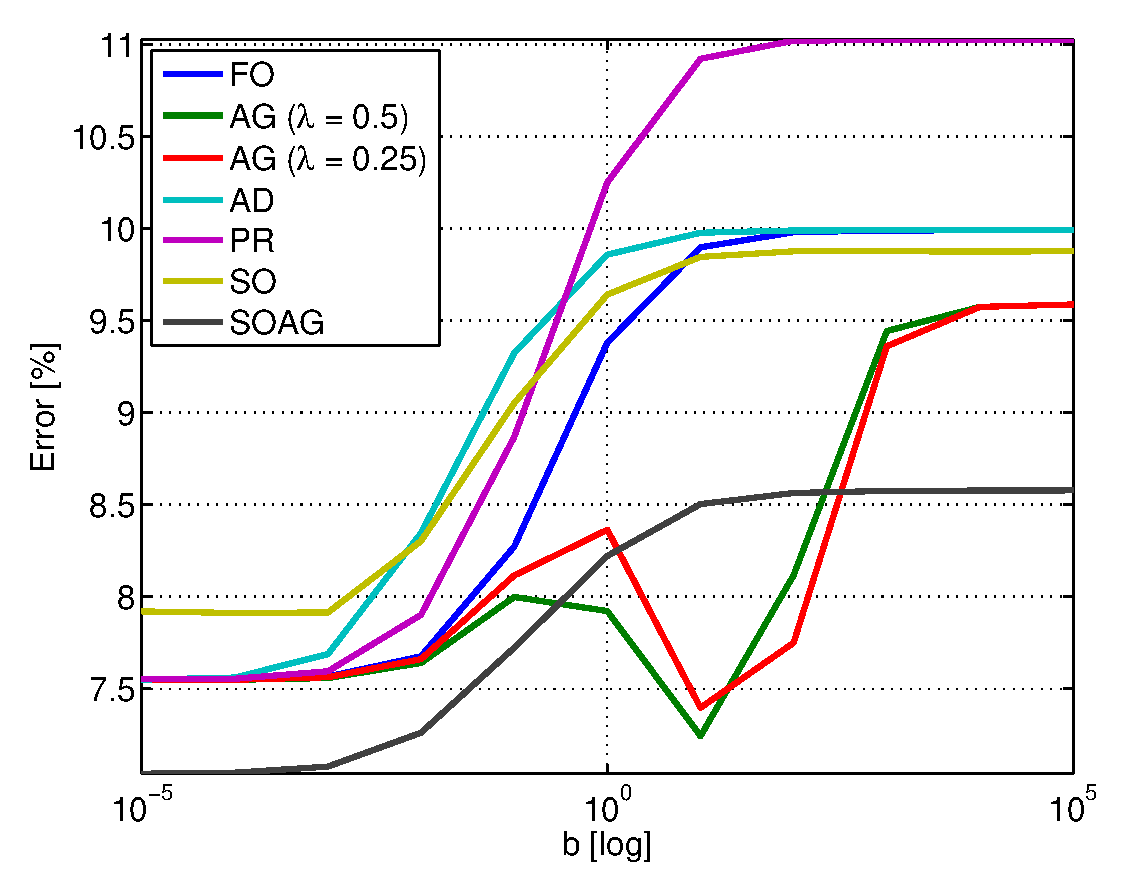
\includegraphics[width=0.4\textwidth]{figs/train-v1.eps}\label{fig:bars1}}
\subfigure[VJ one-vs-rest]{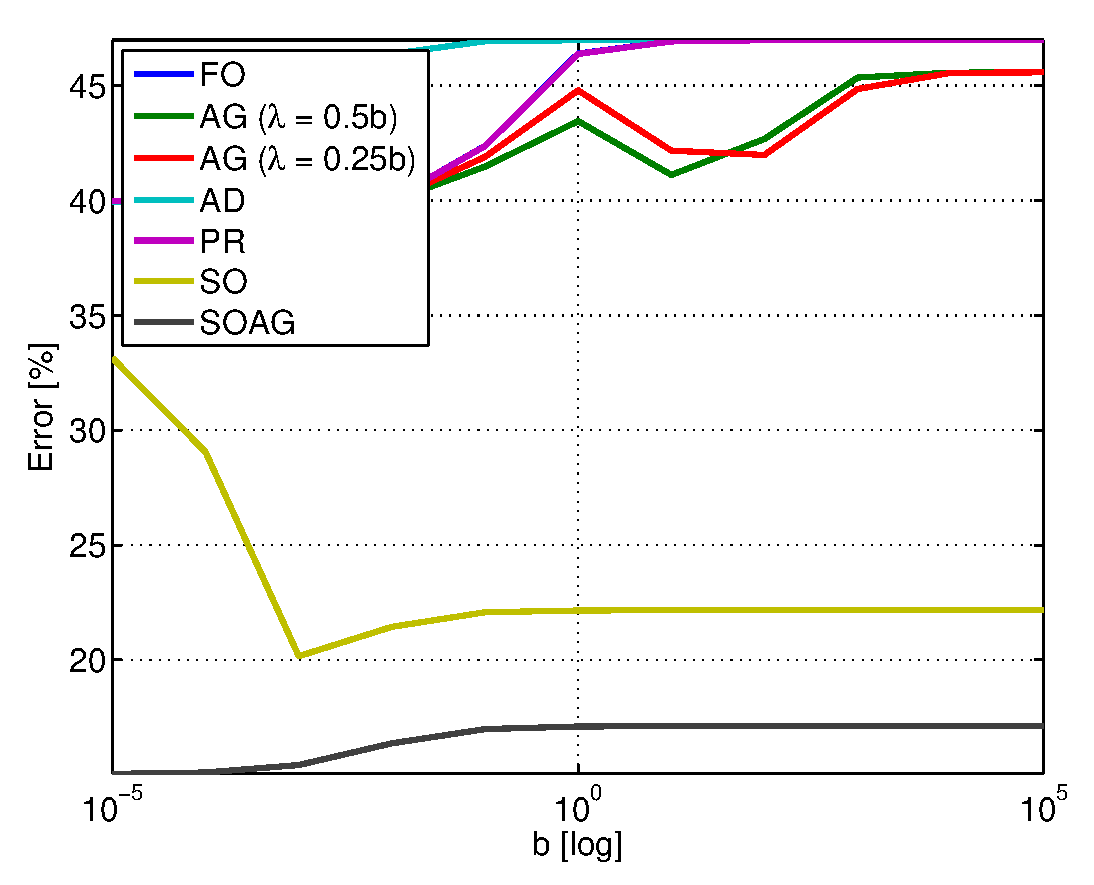
\includegraphics[width=0.4\textwidth]{figs/train-vr.eps}\label{fig:bars2}}
\subfigure[NLP one-vs-one]{\includegraphics[width=0.4\textwidth]{figs/train-n.eps}\label{fig:bars2}}
\caption{train }
\label{fig:train_errors}
\end{centering}
\vspace{-0.5cm}
\end{figure}


\begin{figure}[!t]
\begin{centering}
\subfigure[MNIST one-vs-one]{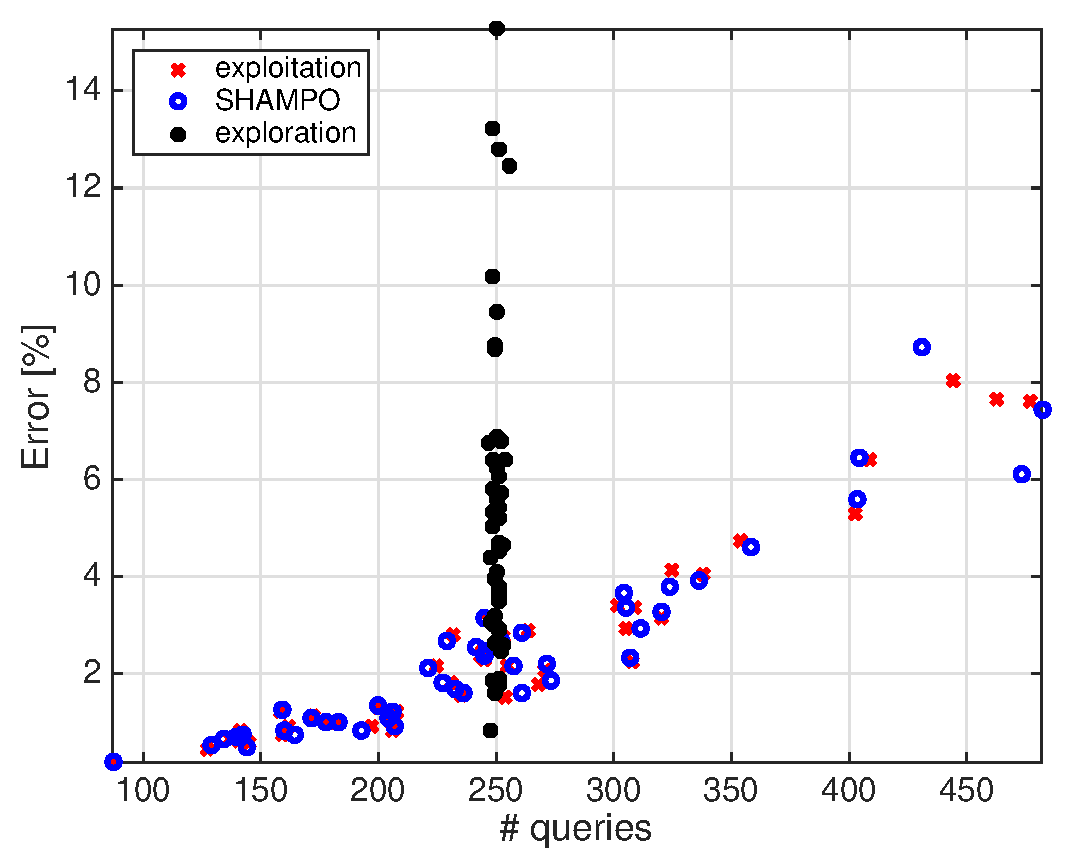
\includegraphics[width=0.4\textwidth]{figs/scatter-m1.eps}\label{fig:scatter_m1}}
\subfigure[MNIST one-vs-rest]{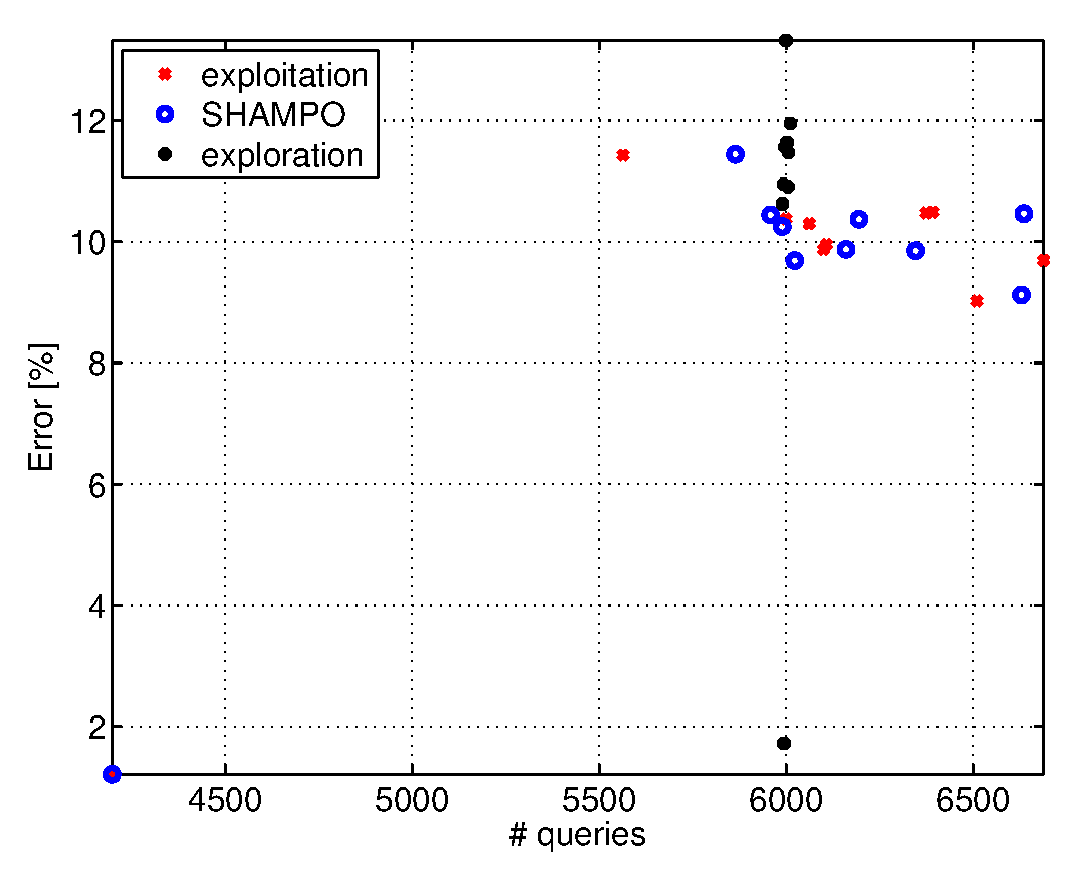
\includegraphics[width=0.4\textwidth]{figs/scatter-mr.eps}\label{fig:scatter_mr}}
\subfigure[USPS one-vs-one]{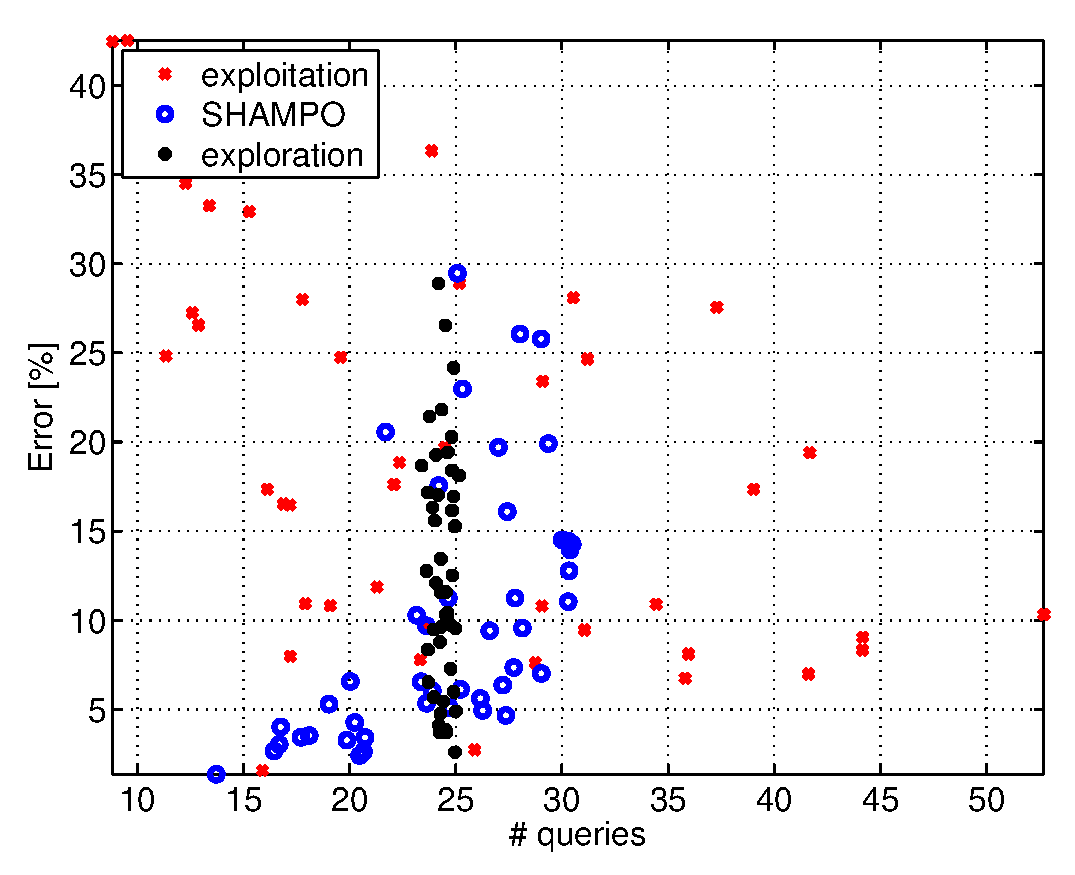
\includegraphics[width=0.4\textwidth]{figs/scatter-u1.eps}\label{fig:scatter_u1}}
\subfigure[USPS one-vs-rest]{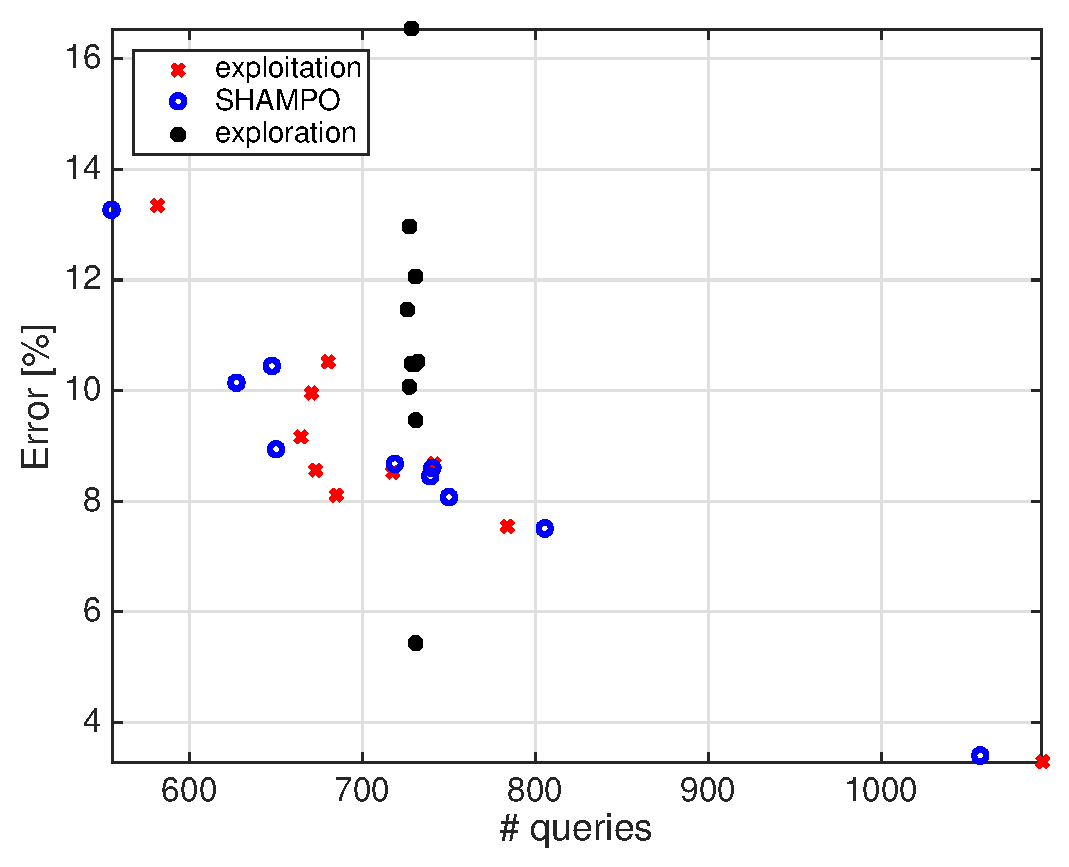
\includegraphics[width=0.4\textwidth]{figs/scatter-ur.eps}\label{fig:scatter_ur}}
\subfigure[VJ one-vs-one]{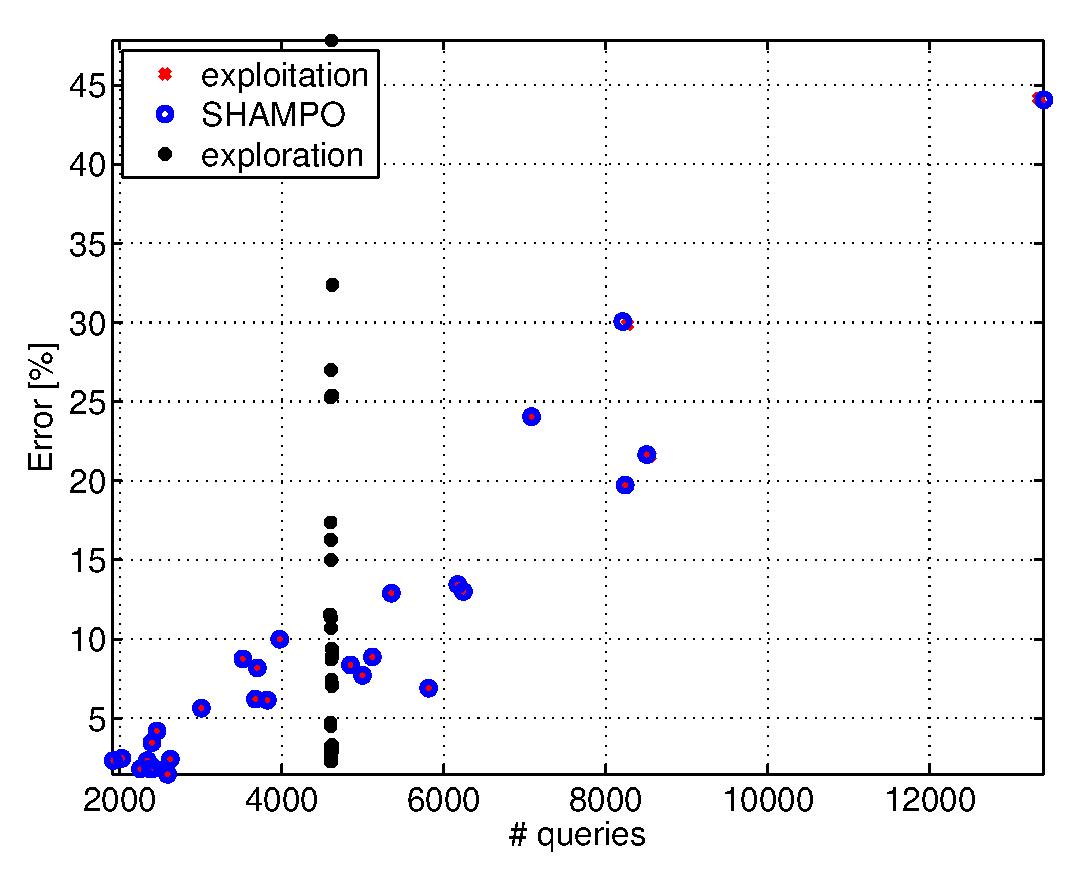
\includegraphics[width=0.4\textwidth]{figs/scatter-v1.eps}\label{fig:scatter_v1}}
\subfigure[VJ one-vs-rest]{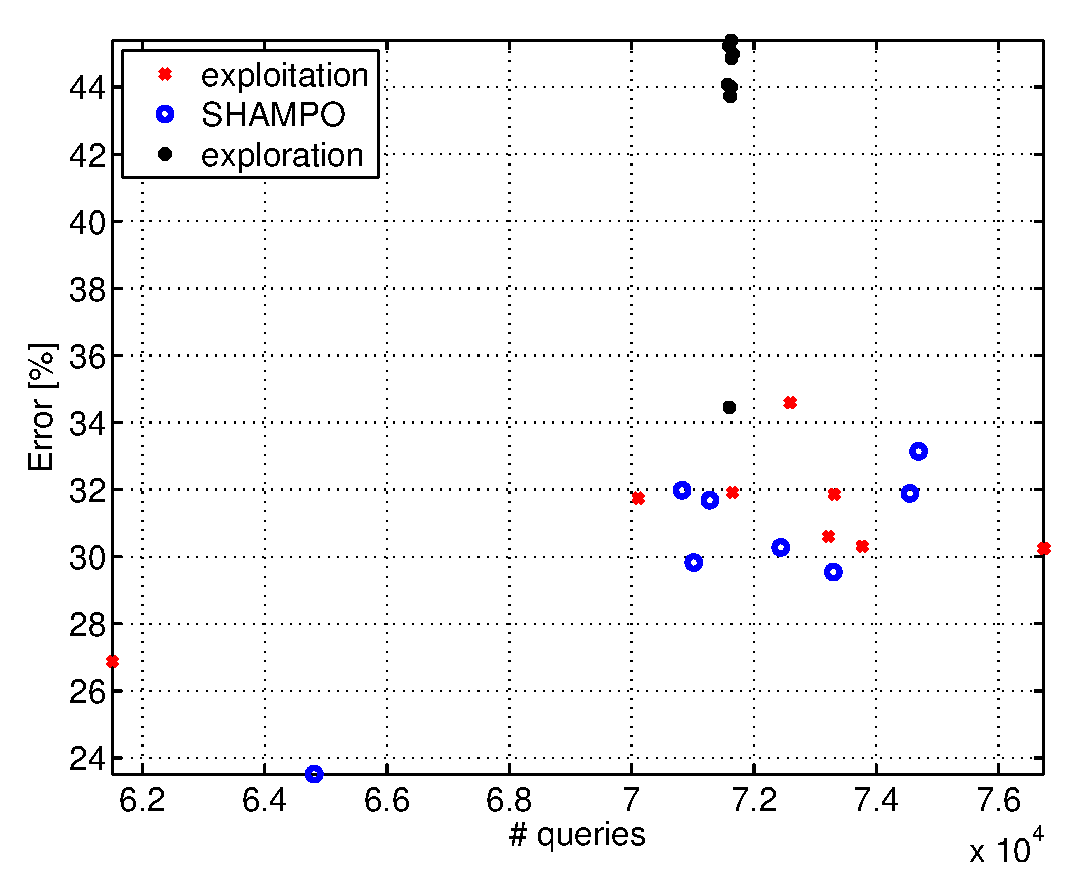
\includegraphics[width=0.4\textwidth]{figs/scatter-vr.eps}\label{fig:scatter_vr}}
\subfigure[NLP one-vs-one]{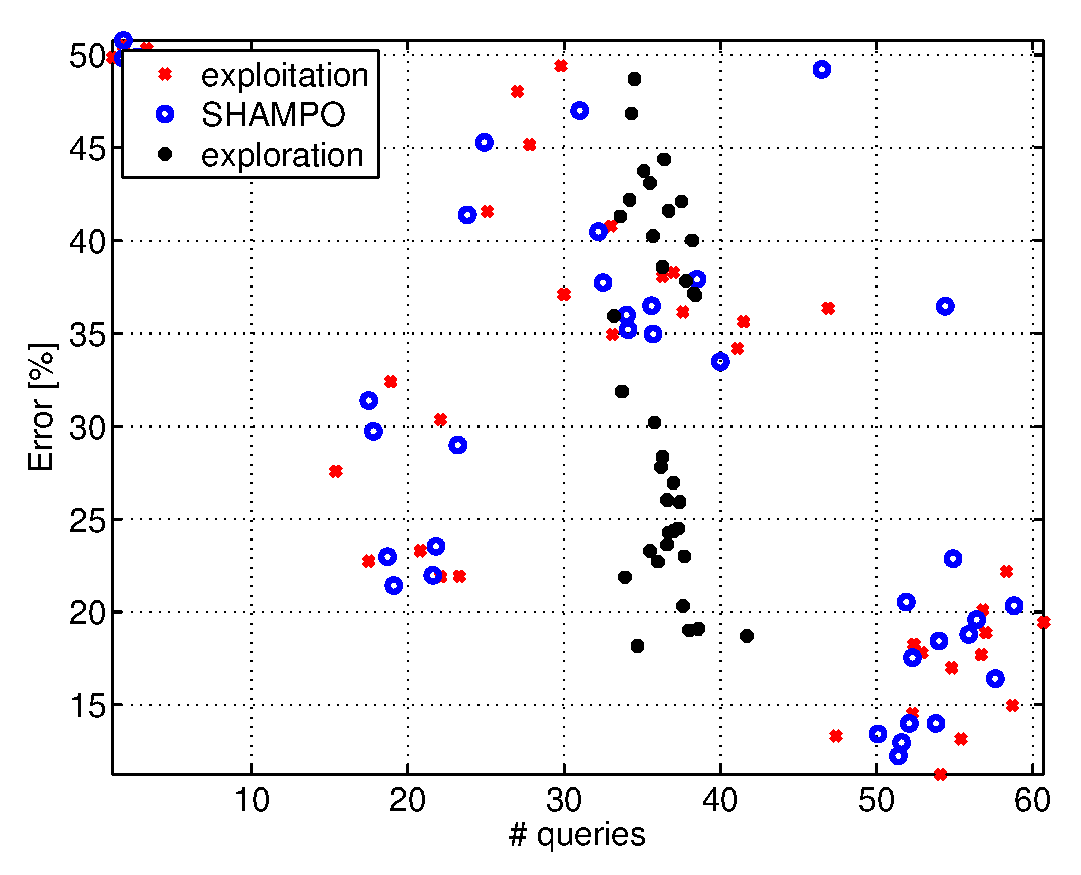
\includegraphics[width=0.4\textwidth]{figs/scatter-n.eps}\label{fig:scatter_n}}
\caption{scatter kjkulk jkhj }
\label{fig:test_scatter}
\end{centering}
\vspace{-0.5cm}
\end{figure}

\section{Reduction of Multi-task to Contextual Bandits}
We also evaluated SHAMPO as a contextual bandit algorithm, by breaking a multi-class problem into few 
binary tasks, and integrating their output into a single multi-class problem. 
We focus on the VJ data, as there are many examples, and linear models perform relatively 
well~\cite{lin2009lose}.  We implemented all three reductions
mentioned in \chapref{chap:multiclass}, namely, {\em one-vs-rest}, {\em one-vs-one-random} which picks a 
random label if the feedback is zero, {\em one-vs-one-weak} (which performs updates to increase 
confidence when the feedback is zero), where we set $\eta=0.2$, and the 
Banditron algorithm~\cite{kakade2008efficient}.
%The results are summarized in \figref{fig:simulations}.
All algorithms show the existence of a tradeoff between exploration and exploitation, 
where {\em one-vs-one-random} is most sensitive to the choice of parameters, yet it also achieves the best 
results, for a large range of values for $b$.
The  {\em one-vs-rest} reduction and the Banditron have a test error of about $43.5\%$, and the 
{\em one-vs-one-random} of about $42.5\%$.
Finally, {\em one-vs-one-weak} achieves an error of $39.4\%$.
 This is slightly worse than PLM
~\cite{lin2009lose} with test error of $38.4\%$ (and higher than MLP with $32.8\%$), 
yet all of these algorithms observe only one bit of feedback per example, while both MLP and PLM 
observe $3$ bits (as class identity can be coded with $3$ bits for $8$ classes). We claim that our setting 
can be easily used to adapt a system to individual user, as we only need to assume the ability to recognize 
three words, such as three letters. Given an utterance of the user, the system may ask: 
``Did you say (a) 'a' like 'bad' (b) 'o' like in 'book') (c) none''. The user can communicate the correct answer 
with no need for a another person to key in the answer.


